\documentclass[11pt]{article}
\newcommand{\numpy}{{\tt numpy}}    % tt font for numpy
\usepackage[margin=1in]{geometry}
\usepackage{hyperref}
\usepackage{graphicx}
\hypersetup{
    colorlinks=true,
    linkcolor=cyan,
    filecolor=magenta,      
    urlcolor=blue,
}

\begin{document}

$$\mbox{\Large \textbf {CS 111 (S19): Homework 4}}$$
$$\mbox{\textbf {Due by 6:00pm Tuesday, April 30}}$$
$$\mbox{\textbf {NAME and PERM ID No.:} Chen Li, 5468137}$$
$$\mbox{\textbf {UCSB EMAIL:} chenli@ucsb.edu}$$

Note: In this homework, you'll be using a few of the functions I introduced in lecture, 
like LSolve, USolve, the temperature setup, etc. These can all be found in our shared 
files GitHub repository of "Useful Files" found
\href{https://github.com/ucsb-cs111/s19-lecture-files/tree/master/UsefulFiles}
{here (link).}

\par\bigskip
{\bf 1.}
The temperature problem models our cabin in the woods in two dimensions,
but most modern scientific simulations are done in three dimensions.
Here you will create the matrix that corresponds to a 3-D version of 
the temperature problem. The ``cabin'' is now the unit cube. As before,
we will discretize the interior by dividing it into $k$ points in each
dimension, but now there are $k^3$ points in all rather than $k^2$.
The partial differential equation still leads to the approximation
that the temperature at any given point is the average of the temperatures
at the neighboring points, but now there are 6 neighbors, 
with $2$ in each dimension.

Using the routine {\tt make\_A(k)} from {\tt Temperature.ipynb} as a model, 
write a routine {\tt make\_A\_3D(k)} that returns the $k^3$-by-$k^3$ 
matrix $A$ for the 3D version of the temperature problem.
This matrix expresses the fact that, in a 3D $k$-by-$k$-by-$k$ grid, 
each interior point has a temperature that is the average of its 6 neighbors 
(left, right, up, down, in, out).
The diagonal elements of $A$ are all equal to $6$, 
and the off-diagonal elements are either $0$ or $-1$.
Most of the rows of $A$ have 7 nonzeros.

Here below, for debugging, is the correct matrix for $k=2$.
I converted it to dense for printing---you should also
print it out as sparse, and indeed for $k>2$ it's going to be too
large to see what's going on in the dense matrix anyway.

\begin{verbatim}
  [In:]
    k = 2
    A = make_A_3D(k)
    print('k:', k)
    print('dimensions:', A.shape)
    print('nonzeros:', A.size)
    #print('A as sparse matrix:'); print(A)
    print('A as dense matrix:'); print(A.todense())

  [Out:]
    k: 2
    dimensions: (8, 8)
    nonzeros: 32
    A as dense matrix:
    [[ 6. -1. -1.  0. -1.  0.  0.  0.]
     [-1.  6.  0. -1.  0. -1.  0.  0.]
     [-1.  0.  6. -1.  0.  0. -1.  0.]
     [ 0. -1. -1.  6.  0.  0.  0. -1.]
     [-1.  0.  0.  0.  6. -1. -1.  0.]
     [ 0. -1.  0.  0. -1.  6.  0. -1.]
     [ 0.  0. -1.  0. -1.  0.  6. -1.]
     [ 0.  0.  0. -1.  0. -1. -1.  6.]]
\end{verbatim}

Print out your matrix for $k=2$ and $k=3$ as a check that it's correct. 
Also use {\tt plt.spy(A)} to make a spy plot of the nonzero structure 
for $k=4$ or $5$ (you may want to zoom in on the plot to see all the structure).

To complete a realistic simulation you would also 
write a routine {\tt make\_b\_3D(k)} to compute the right-hand side $b$.
For this problem, you don't have to do that; 
for the experiments in Problem 2 you can just use {\tt np.random.rand()}
to generate a random $b$.

{\bf Note}:
When you finish, submit your code of {\tt make\_A\_3D(k)} to Gradescope.
The file name must be {\tt make\_A\_3D.py}.
The function name must be {\tt make\_A\_3D}.
A \href{https://github.com/ucsb-cs111/s19-lecture-files/blob/master/04.23/make_A_3D.py}
{skeleton code file} can be found in 04.23 lecture files.
\newpage

\par\bigskip
{\bf 2.} 
Now you will experiment with solving $At=b$ using various solvers
from class and from {\tt numpy}.
For this problem, you should use the 3-D version of the temperature matrix
from Problem 1. 
(You can get partial credit by using the 2-D temperature matrix from the
class instead.)
You can use a randomly chosen right-hand side vector $b$.

Experiment with solving $At=b$ for the temperature $t$, 
for various values of $k$, using five different solvers:
\begin{itemize}
\item The {\tt CGsolve()} conjugate gradient solver, from class.
(You can vary the arguments {\tt tol} and {\tt max\_iters} to
make it find a more accurate solution.)
\item The {\tt Jsolve()} Jacobi solver, also from class.
(Again you can vary {\tt tol} and {\tt max\_iters}.)
\item The {\tt scipy} sparse conjugate gradient solver {\tt spla.cg()}.
\item The {\tt scipy} sparse LU solver {\tt spla.spsolve()}.
\item The {\tt LUsolve()} dense LU solver from class.
(For this, you will have to use the dense form of $A$ that you get
from {\tt A.todense()}. Warning! This will use too much memory if
$k$ gets very big at all.)
\end{itemize}
For each solve, measure the run time and also the relative residual norm.
Which solvers are more accurate? Which are faster? How do the
answers to these questions change as you change $k$?

Warning: Start with very small values of $k$, and be cautious
as you increase $k$!
The matrices get big in a hurry.
Different solvers will fall over for different values of $k$;
try to see how big a value of $k$ each solver can handle with
at most 30 seconds of compute time. 
\\\\k were set as 5, 10, 20, 30, 40, 50, the tolarance were set to $10^{-15}$, and all the max iteration were set base on when the relative residual is smallest to find the executing time accurately.\\\\when k = 5, spla.spsolve is fastest and most accurate, Jsolve and LUsolve are relatively solwer but also accurate engouth. However, CGsolve is the only one can't reach tolerance of $10^{-15}$\\For spla.cg tolerance are tentative to find the best performance and accuracy because slight if tolerance higher than possible result, it will extremely long time to execute. 
\\\\when k = 10, spla.cg reach its most accurate point (relres = 3.88e-15) within first 100 iteration but then can't go closer. Therefore, it took more than 4 second to execute just for go through 10000 iterations. so I start to  adjust it tolerance. Jsolve go very close to tolerance(relres = 1.09e-15). Jsolve and LUsolve is still very slower
\\\\when k = 20, spla.cg is not accurate(relres=7.72e-14)but very fast. Jsolve is accurate(relres=3.79e-15) but slow.CGsolve were set to 200 iteration and reach its maximum accuracy(relres=2.63e-14), which take slightly longer than spla.cg. For LUsolve, it takes too long I decided to interupte it.\\\\
when k = 30, spla.cg is still the fastest but not accurate, Jsolve is slow but accurate. Others are in between.\\\\
when k = 50, Jsolve take more than 30 seconds, CGsolve this time reaches its accurate place in 1.37 second, but is not accurate(relres=2.42e-13) comparing with spla.cg, which take slightly longer to reach one more decimal place. Only these two left for now.\\\\
when k = 70, all solvers need more than 30 second, so I have to adjust tolerance to e-12 to compare. CGsolve is slightly faster and spla.cg is slightly accurate in this case.\\
\\here is the structure of the code I use to measure\\
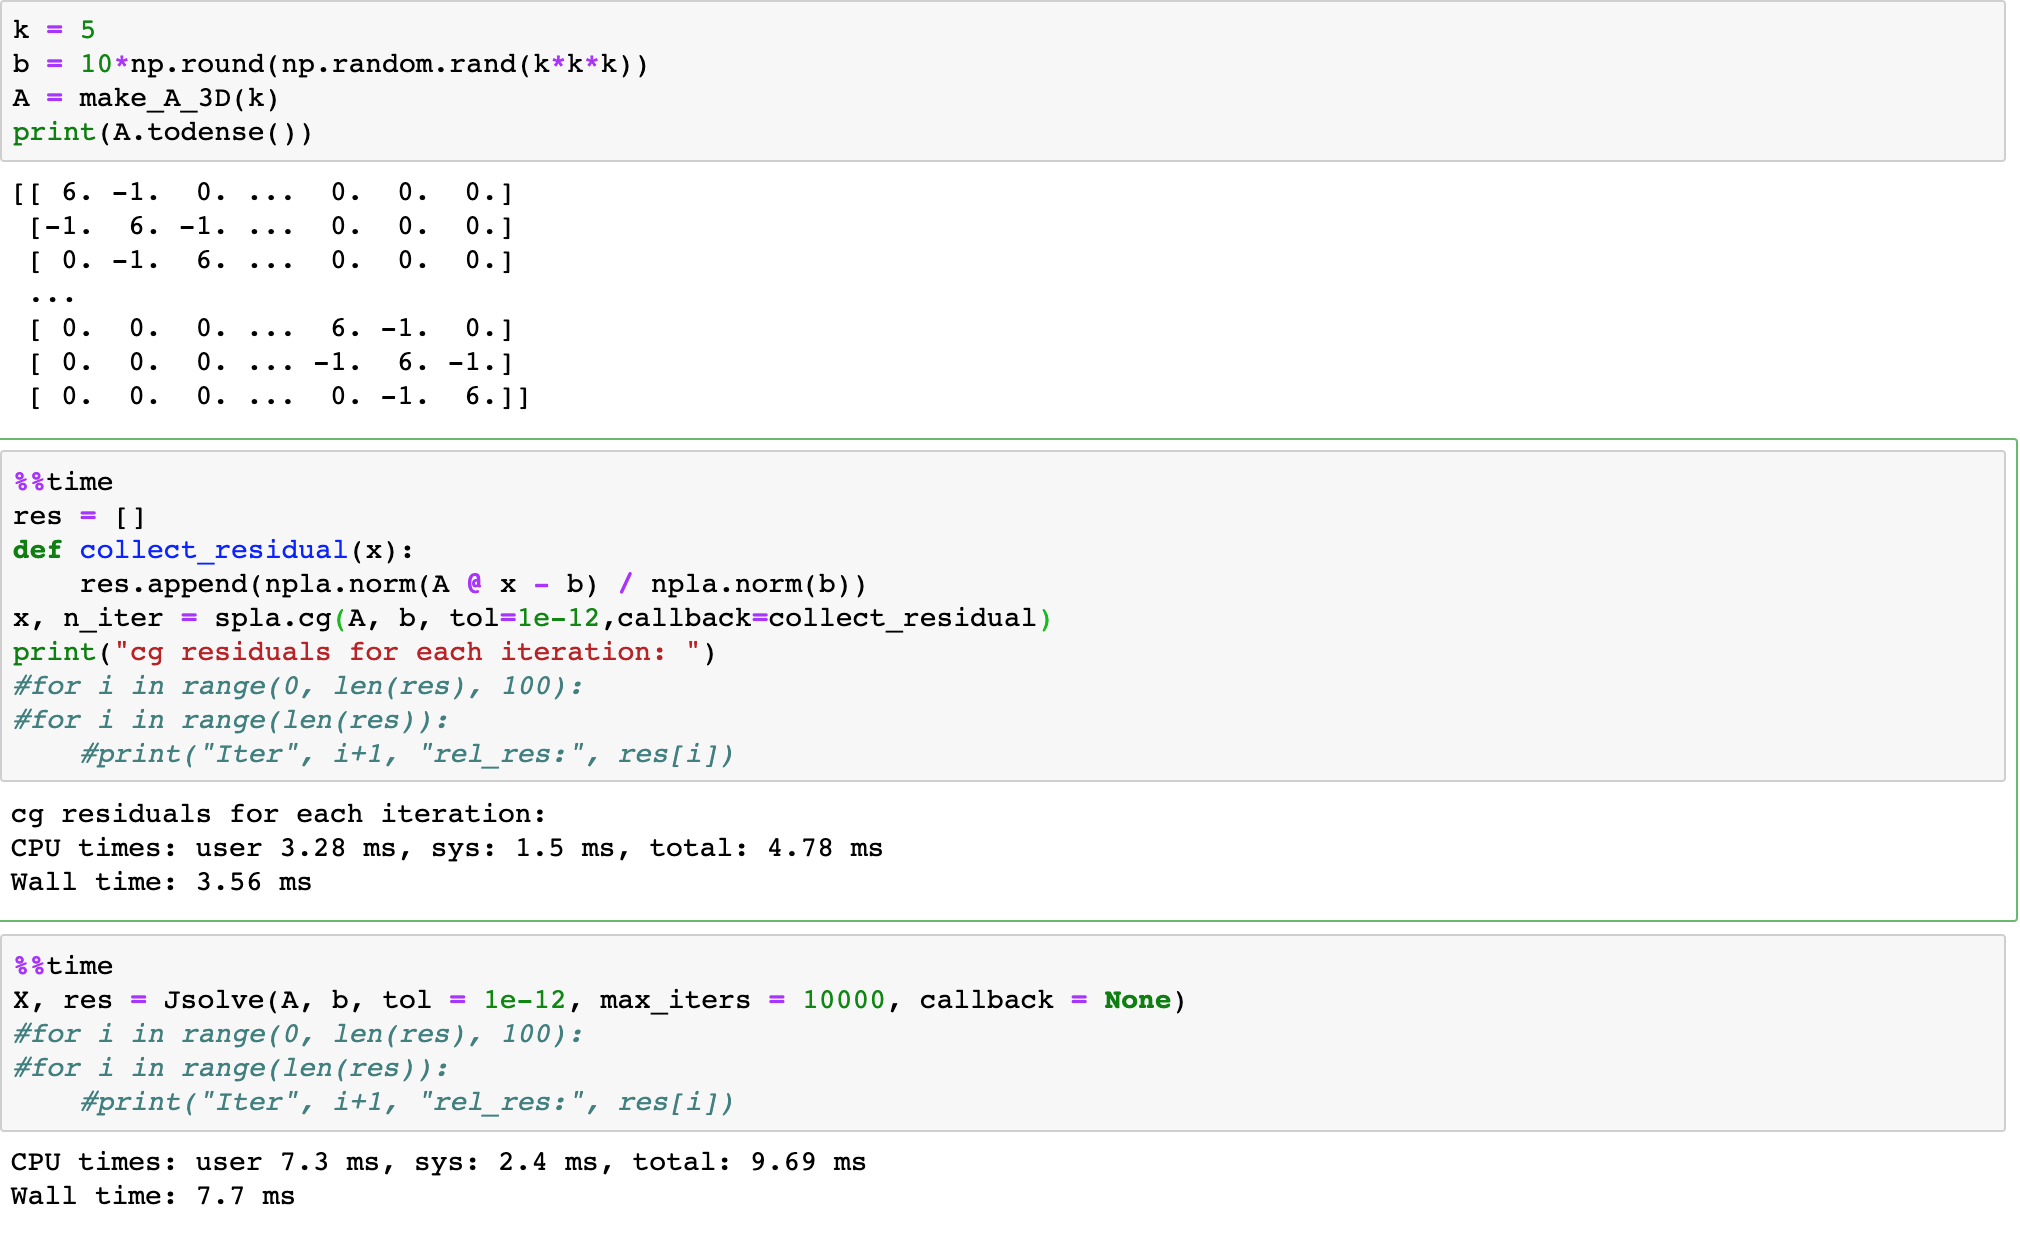
\includegraphics[scale=0.4]{H421}\\
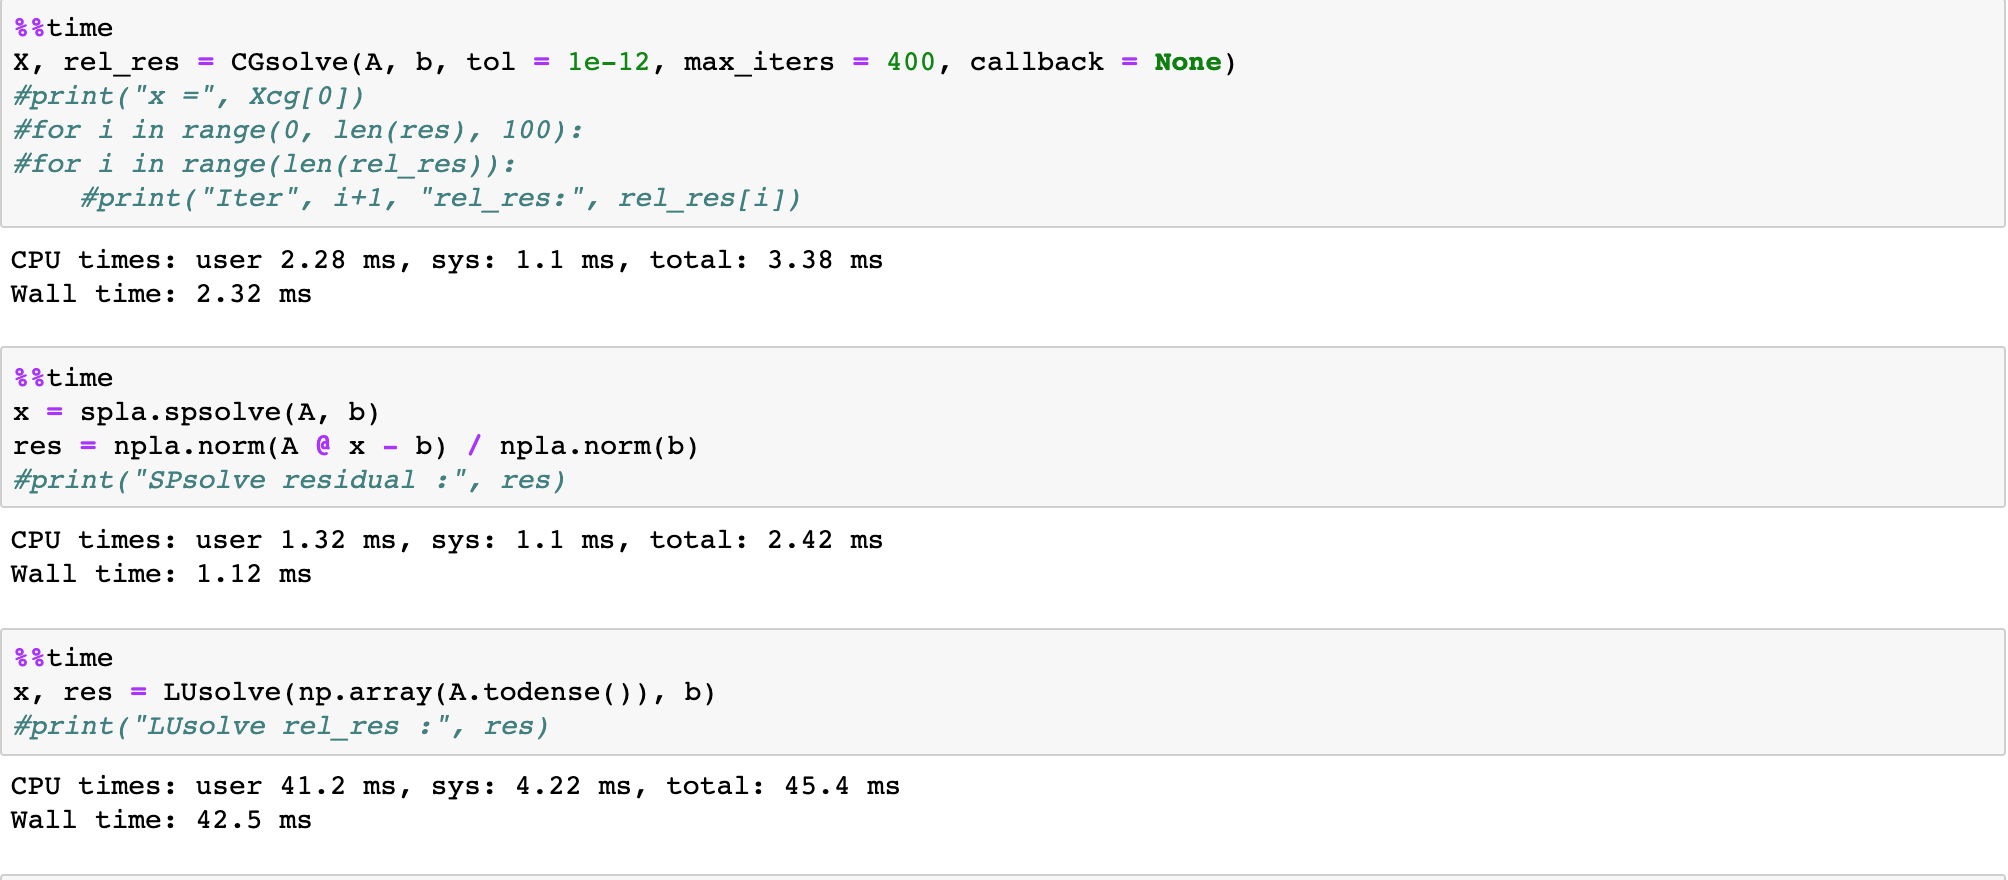
\includegraphics[scale=0.4]{H422.png}\\here is the result record\\
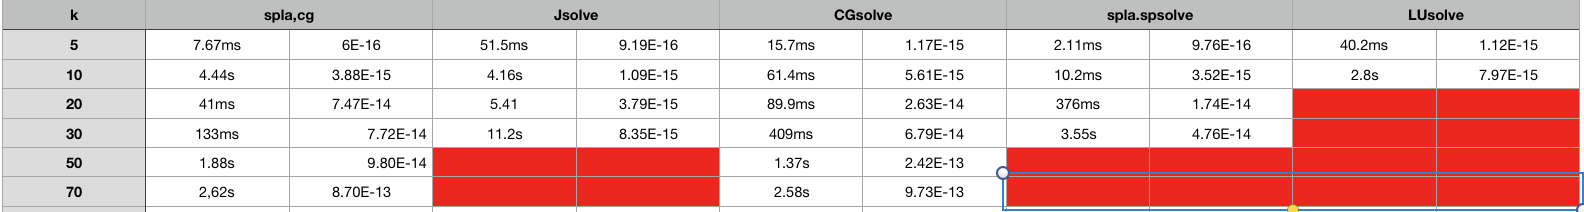
\includegraphics[scale=0.6]{H423.png}\\
As a conclusion, Jsolve, and spla.spsolve are accurate but slow. CGsolve and cpla.cg are fast but lack of accuracy, which require to adjust to larger tolerance to get use. Since the matrix is SPD, the result for two cg solvers are reasonable.


\par\newpage
{\bf 3.} 
Let
$$A =
   \left(
   \begin{array}{ccc}
    4 & -1 & -1 \\ 	
   -1 &  4 & -1 \\ 
   -1 & -1 &  4 \\
   \end{array} \right)
$$
and let $b = (15, -3, 12)^T$.

\par\medskip
{\bf 3a.}
Use the {\tt scipy} Cholesky factorization routine {\tt linalg.cholesky()}
to compute the triangular Cholesky factor of $A$.
(Either upper or lower triangular is fine, but just compute one of them.)
Verify that the answer is correct by multiplying the factor by its transpose and
comparing with $A$.
Then use {\tt Usolve()} and/or {\tt Lsolve()} to compute the solution $x$
to $Ax=b$ from the Cholesky factor (without calling any other factorization routine).
Show the Jupyter/Python input and output for your computations.\\
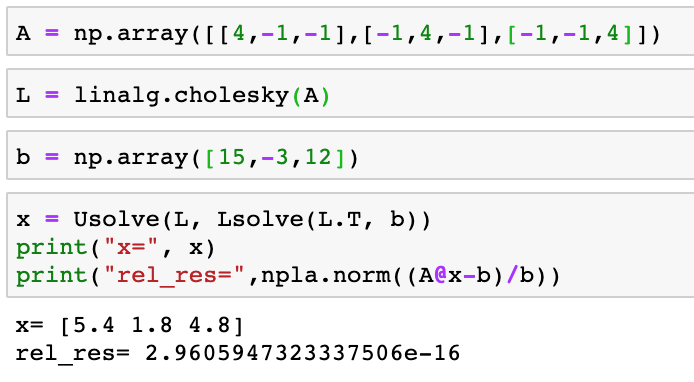
\includegraphics[scale=0.8]{H4_3a}\\
\par\medskip
{\bf 3b.}
Use the {\tt scipy} QR factorization routine {\tt linalg.qr()}
to compute the two matrices (orthogonal and upper triangular) that
constitute the QR factorization of $A$.
Verify that the answer is correct by multiplying the factors and comparing with $A$.
Then use {\tt Usolve()} and/or {\tt Lsolve()} to compute the solution $x$
to $Ax=b$ from the QR factors (without calling any other factorization routine).
Show the Jupyter/Python input and output for your computations.\\\\
$Ax=b\Rightarrow QRx=b\Rightarrow Rx=Q^Tb$, then we can use Usolve\\
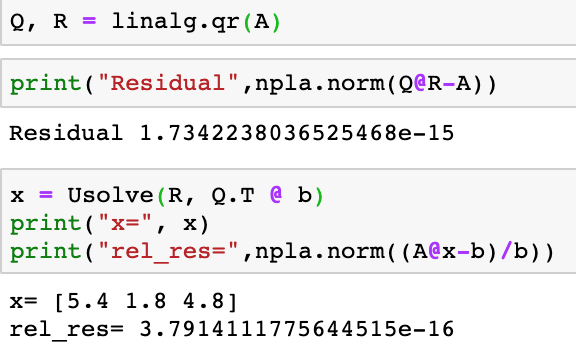
\includegraphics[scale=0.8]{H4_3b.png}\\
\newpage
\par\bigskip
{\bf 4.}
How do you define an orthogonal matrix? 

Which of the following matrices are orthogonal?
(Don't show your work, just give the answer.)
$$
   A =
   \left(
   \begin{array}{cc}
    0 & 1 \\ 	
    1 & 0 \\ 
   \end{array} \right), 
   \hspace{10pt}
   B =
   \left(
   \begin{array}{cc}
    1 & 0 \\ 	
    0 & -1 \\ 
   \end{array} \right), 
   \hspace{10pt}
   C =
   \left(
   \begin{array}{cc}
    2 & 0 \\ 	
    0 & 1/2 \\ 
   \end{array} \right), 
   \hspace{10pt}
   D =
   \left(
   \begin{array}{cc}
    \sqrt 2 / 2 & \sqrt 2 / 2 \\ 	
    -\sqrt 2 / 2 & \sqrt 2 / 2 \\ 	
   \end{array} \right)
$$
a matrix Q is a orthogonal matrix means its columns are pair-wise orthonomal with norm of one unit, and its rows are pair-wise orthonomal: $QQ^T = Q^TQ=I$ and $Q^T=Q^{-1}$\\
A, B, D are orthogonal

\end{document}
